\documentclass[12pt,fleqn]{article}\usepackage{../common}
\begin{document}
Ders 4

Bu derste yapacaklarimiz sunlar; bir $AB$ carpiminin tersini (inverse)
nasil alirim? Biliyoruz ki 

\[ AA ^{-1}  = I = A ^{-1} A \]

Soru su ki 

\[ AB... = I \]

noktali kisma ne gelirse sonuc birim (identity) matris olur? Sonra bu
bilgiyi bir baska carpim uzerinde kullanacagiz, bu carpim eliminasyon
matrislerini bir sira carpim olarak gorecek, ve bu sekilde Gaussian
eliminasyon islemine degisik bir bakis getirmis olacagiz. 

$AB$'den birim matrise nasil erisirim? 

\[ ABB ^{-1} A ^{-1} = I \]

Ya da

\[ B ^{-1}A ^{-1} AB  = I\]

Simdi tersini alma isleminin devrigini alma ile nasil isleyecegine
bakalim. Diyelim ki 

\[ AA ^{-1} = I \]

Bunun tersini alirsam ne olur ?

\[ (A ^{-1})^T A^T = I \]

Devrik alinca siralama degisiyor bildigimiz gibi, ve birim matrisin devrigi
yine kendisi. 

Fakat ustteki ifade bir seyi daha soyluyor: $A^T$'yi ne carparsa sonuc $I$
gelir? Cevap $A^T$'nin tersi! Yani $(A ^{-1})^T$ ve  $(A^T) ^{-1}$
ifadelerinin ayni sey oldugunu soylemis oluyoruz. Bu nasil kullanilabilir?
Eger $A^T$'nin tersini hesaplamamiz gerekiyorsa, ve $A$'nin tersini bir
sekilde biliyorsam, onun devrigini almam yeterli. Diger bir deyisle,
tersini alma ve devrigini alma islemleri herhangi bir sirada yapilabilir. 

Eliminasyona gelelim.

Onlar bir matrisi anlamanin dogru yoludur denebilir. $A = LU$
faktorizasyonu bir matrisi en temel parcalarina ayirir. Diyelim ki $A$'dan
basliyorum, hic satir degis tokusu yapmadan sadece eliminasyon yaparak
ilerliyorum, ve $U$'ya erisiyorum, pivotlarimin hicbir sifir degil. Bu iki
matris arasindaki baglanti nedir? $A$ ile $U$ nasil alakali? Simdi
gorecegimiz uzere aradaki baglanti $L$. 

Ornek

\[ \stackrel{A}{
\left[\begin{array}{rr}
2 & 1 \\ 8 & 7
\end{array}\right]
}
 \]

$U$'ya yani bir ust ucgenel matrise (upper triangular matrix) erismek
istiyorum, 1. satirin 4 katini 2. satirdan cikartirim. Bu isleme 2'den 
1 ciktigini sembolize etmek icin $E_{21}$ adini verelim, 

\[ 
\stackrel{E_{21}}{
\left[\begin{array}{rr}
1 & 0 \\ -4 & 1
\end{array}\right]
}
\stackrel{A}{
\left[\begin{array}{rr}
2 & 1 \\ 8 & 7
\end{array}\right]
}
=
\stackrel{U}{
\left[\begin{array}{rr}
2 & 1 \\ 0 & 3
\end{array}\right]
}
 \]

O zaman sunu yazarsak, 

\[ 
\stackrel{A}{
\left[\begin{array}{rr}
2 & 1 \\ 8 & 7
\end{array}\right]
}
=
\stackrel{L}{
\left[\begin{array}{rr}
 &  \\  & 
\end{array}\right]
}
\stackrel{U}{
\left[\begin{array}{rr}
2 & 1 \\ 0 & 3
\end{array}\right]
}
 \]

$L$ diyen yere ne gelmeli? Basit, $E_{21}$'nin tersi gelmeli. $E_{21}A =
U$'yu 
$A=LU $ yapmak icin her iki tarafi soldan $E_{21}$'nin tersi ile
carparim, esitligin solunda  $E_{21}$ yokolur, sagina tersi gelir, yani bana $E_{21}$'nin 
tersi gerekli. 

Hatirlarsak, eliminasyon matrislerinin tersini almak kolaydir,

\[ 
\stackrel{A}{
\left[\begin{array}{rr}
2 & 1 \\ 8 & 7
\end{array}\right]
}
=
\stackrel{L}{
\left[\begin{array}{rr}
1 & 0 \\ 4 & 1
\end{array}\right]
}
\stackrel{U}{
\left[\begin{array}{rr}
2 & 1 \\ 0 & 3
\end{array}\right]
}
 \]

$L$ alt ucgensel (\textbf{l}ower triangular) demek, $U$'nun kosegeninde
pivotlar var, sol alt kisminda sifirlar var. Esitligin sagindaki $L$ icinden
pivotlari cikartmak mumkun, mesela 2'yi ve 3'u cekip cikartirsak, 

\[ 
=
\left[\begin{array}{rr}
1 & 0 \\ 4 & 1
\end{array}\right]
\left[\begin{array}{rr}
2 & 0 \\ 0 & 3
\end{array}\right]
\left[\begin{array}{rr}
1 & 1/2 \\ 0 & 1
\end{array}\right]
 \]

Bu sonuca $LDU$ denebilir, Matlab her iki sonucu da uretebilmektedir. 

Eger 3 boyutta olsaydik ne yapardik? Once $E_{21}$, sonra $E_{31}$,
vs. Hepsi bir arada

\[ E_{32}E_{31}E_{21} A = U\]

Diyelim ki tum bu eliminasyon $E$ matrislerini esitligin saginda
istiyorum. Yani

\[ A = ....U \]

noktalara ne gelecek? 

\[ A = E_{21} ^{-1}  E_{31} ^{-1}  E_{32} ^{-1}  U\]

ve bu terslerin tamamina $L$ diyebiliriz. Ilginc bir sey, terslerin
carpimi ile calismak, eliminasyon matrislerinin carpimiyla calismaktan daha
kolay. Niye?

Ornek

\[ 
\stackrel{E_{32}}{
\left[\begin{array}{rrr}
1 & 0 & 0 \\
0 & 1 & 0 \\
0 & -5 & 1
\end{array}\right] }
\stackrel{{E_{21}}}{
\left[\begin{array}{rrr}
1 & 0 & 0 \\
-2 & 1 & 0 \\
0 & 0 & 1
\end{array}\right]}
 \]

Bu carpimi yaptigimizda sonucun ilk kismini hemen goruyoruz, ustte
sifirlar, kosegende 1'ler var.

\[ = 
\left[\begin{array}{rrr}
1 & 0 & 0 \\
 & 1 & 0 \\
 &  & 1
\end{array}\right]
 \]

Geri kalanlar? 

\[ = 
\left[\begin{array}{rrr}
1 & 0 & 0 \\
-2 & 1 & 0 \\
10 & -5 & 1
\end{array}\right]
 \]

Fakat ustteki su 10 rakami beni rahatsiz ediyor. 

Once $E_{21}$'in tersiyle baslayalim, tersi matrisin aynisi, sadece eksiler
arti oluyor, sonra  $E_{32}$'nin tersi

\[ 
\left[\begin{array}{rrr}
1 & 0 & 0 \\
-2 & 1 & 0 \\
0 & 0 & 1
\end{array}\right]
\left[\begin{array}{rrr}
1 & 0 & 0 \\
0 & 1 & 0 \\
0 & -5 & 1
\end{array}\right]
=
\left[\begin{array}{rrr}
1 & 0 & 0 \\
2 & 1 & 0 \\
0 & 5 & 1
\end{array}\right] = L
 \]

Iste bu sagdaki matris aradigimiz $L$. 

\[ EA = U \]

\[ A = LU \]

Bakiyoruz ki $L$ matrisinde 10 gibi bir sayi yok. Bunun sebebi $L$'i
olusturan carpimlarin ``dogru matrisler'' olmasi. Hicbir satir degisimi
yok, o zaman carpanlar direk $L$'e dahil oluyorlar. 

Simdi su soruyu soralim? Eliminasyon ne kadar pahali bir islemdir? Ilk once
sol kismi sifirlamak gerekir, pivot en ust sol kosedir, vs.

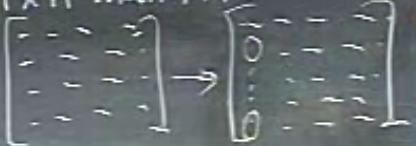
\includegraphics[height=2cm]{01.png}

Eger $n=100$ ve $n \times n$ bir sistemimiz olsa, kac tane operasyon yapmamiz
gerekir? Bu islem bir  $n \times n$ matrisin bir diger  $n \times n$ matris ile
carpilmasini gerektirdigi icin $100^2$ islem lazim. Sonra geri kalan
bolgede benzer islemi yaparim (altta hoca yuvarlak ile isaretledi)

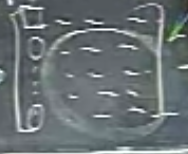
\includegraphics[height=3cm]{02.png}

bu islemler yaklasik $99^2$ tanedir. Toplam

\[ n^2 + (n-1)^2 + ... + 1^2 \approx \frac{ 1}{3} n^3 \]

Ustteki sonucu kabaca soyle dogrulamak mumkundur, mesela Calculus'ta
$x^2$'nin entegralini aliyor olsaydik, sonuc $x^3/3$
cikardi. Ustte ise 1 ile n arasindaki sayilarin karesini ``topluyoruz'' ve
bu ayriksal bir islem, ama zaten Calculus'ta entegraller, ayriksal toplam
isleminin karsiligi degil midirler? 

Bu $A$ uzerindeki islemlerin yuku. Eliminasyon islemleri yapilirken bir de
$A$'nin yaninda tutulan ve ayni islemlerin uygulandigi bir $b$ kolonu da
var, ayrica bu kolonu sonra geriye denklemlere sokuyoruz
(backsubstitution). Onun getirdigi islem yuku $n^2$.

Bu tartistigimiz lineer bir denklem sistemini cozmek icin kullanilan en
temel algoritmadir. Cok onemli bir konu. 

Eger satir degisimi olsaydi, ne olurdu? Pivot pozisyonunda sifir degeri
varsa, satir degisimi yapmak sart. 

Satir degisimi permutasyon oldugu zaman da devreye girer. Mesela $3 \times
3$ baglaminda dusunursek, hicbir degisim yapmayan permutasyon matrisi birim
matristir, yani 

\[ 
\left[\begin{array}{rrr}
1 && \\
 & 1 & \\
 && 1
\end{array}\right]
 \]

Eger 1 ile 2'yi degistirmek istesem? Bir tiyo: istedigim permutasyon,
degistirici matrisi elde etmek icin, istedigim degisimi birim
matrisi uzerinde gerceklestiririm, ve bu matrisi hangi diger matrisle
carparsam gerekli satir degisimi onun uzerinde gerceklesir. 

\[ P_{12} = 
\left[\begin{array}{rrr}
0 & 1 & 0\\
1 & 0 & 0 \\
0  & 0 & 1
\end{array}\right]
 \]

\[ P_{13} = 
\left[\begin{array}{rrr}
0 & 0 & 1\\
0 & 1 & 0 \\
1  & 0 & 0
\end{array}\right]
 \]

\[ P_{23} = 
\left[\begin{array}{rrr}
1 & 0 & 0\\
0 & 0 & 1 \\
0  & 1 & 0
\end{array}\right]
 \]

Diger bazi matrisler, 

\[  
\left[\begin{array}{rrr}
0 & 1 & 0\\
0 & 0 & 1 \\
1  & 1 & 0
\end{array}\right]
 \]

\[  
\left[\begin{array}{rrr}
0 & 0 & 1\\
1 & 0 & 0 \\
0  & 1 & 0
\end{array}\right]
 \]
 
Toplam 6 tane. Eger bu matrislerin ikisini birbiriyle carpsam ne olur?
Sonuc yine ustteki liste icinde olmalidir. Tersini alirsam, yine ayni
sekilde. Mesela $P_{12}$'nin tersi nedir? Hangi carpim bu matrisi birim
matrisi yapar sorusunu soralim, ama zaten bu matrisi birim matrisi uzerinde
degisim ile elde etmemis miydik? O zaman ayni degisimi bir daha yaparsak
birim matrisi elde ederiz, yani $P_{12}$'nin tersi kendisidir. 

Permutasyon matrisleri hakkinda bir gercek daha, tersi islemi devrik islemi
ile aynidir, yani $P ^{-1}  = P ^{T} $. 

$4 \times 4$ icin 24 tane permutasyon var, vs.


\end{document}
